\documentclass{article}
\usepackage{graphicx}
\usepackage{hyperref}
\usepackage{caption}
\usepackage{subcaption}
\usepackage[dutch]{babel}

\begin{document}

\begin{center}
	\huge{Wiskunde in Kunst}\\
	\LARGE{Opdracht 1} \\
	
	\vspace{2cm}
	
	\Large{Circle Limit III}\\
	\large{\textit{M. C. Escher}}
	
	\begin{figure}[htp]
		\centering
		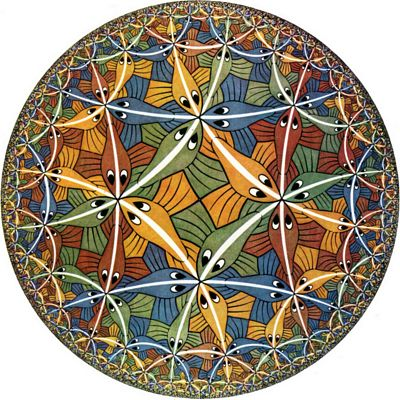
\includegraphics[scale=1.00]{Escher_Circle_Limit_III.jpg}
		\label{}
	\end{figure}
	
	\vfill
	\Large{Marcelo Dias Avelino} \hfill \large{0840416}
\end{center}

\pagebreak

\section{Kunstwerk}

De kunstwerk \textit{Circle Limit III} is een houtsnede stuk gemaakt door de nederlandse kunstenaar Maurits Cornelis Escher (meestal gerefereerd als M. C. Escher). Escher heeft dit kunstwerk gemaakt in 1959 in zijn huis in Baarn, Utrecht. Hij verhuisde hierheen in 1941 vanuit Brussel vanwege de tweede wereld oorlog. Hier heeft hij de grootste gedeelte van zijn meest bekende kunstwerken, zoals \textit{Drawing Hands}, \textit{Relativity} en \textit{Waterfall}.

\begin{figure}[h]
        \centering
        \begin{subfigure}{0.33\textwidth}
                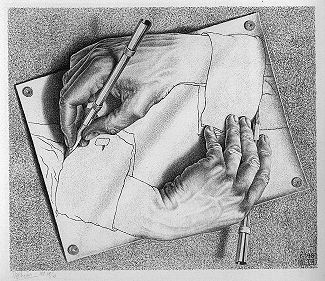
\includegraphics[width=\textwidth]{DrawingHands}
                \caption{\textit{Drawing Hands}}
        \end{subfigure}%
       	~ 
        \begin{subfigure}{0.33\textwidth}
                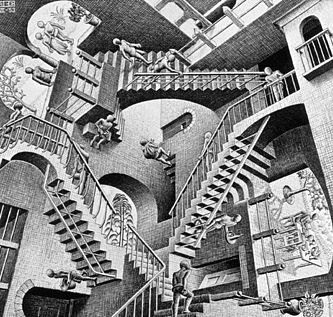
\includegraphics[width=\textwidth]{Escher's_Relativity}
                \caption{\textit{Relativity}}
        \end{subfigure}%
        ~ 
        \begin{subfigure}{0.33\textwidth}
                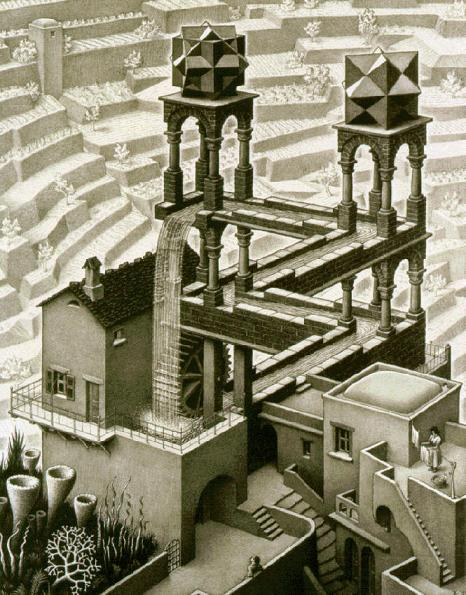
\includegraphics[width=\textwidth]{Escher_Waterfall}
                \caption{\textit{Waterfall}}
        \end{subfigure}%
        \caption{Drie bekende kunstwerken van Escher.}
        \label{fig:structCompare}
\end{figure}

\noindent Escher's inspiratie voor de \textit{Circle Limit III} kwam van een bezoek aan Alhambra. Alhambra is een paleis in Spanje waar muren te vinden zijn die versierd zijn met repetitieve patronen die elkaar niet mogen overlappen, zo genaamd tesselatie of betegeling. Dit kunstwerk is verder ook gebaseerd op een afbeelding die zich bevond in een paper van meetkundiger Donald Coxeter genaamd \textit{``Crystal Symmetry and its Generalizations''}. De afbeelding, die te zien is in Figuur \ref{fig:hyperbolic-domains}, weergeeft een tesselatie met rechthoekig driehoeken met hoeken van 30, 45, and 90 graden binnen een hyperbolische vlakte. 

Een hyperbolische vlakte, in dit geval is het een halve sfeer, is een vlakte waar twee parallel lopende lijnen steeds verder weg van elkaar buigen hoe verder je elke kant op gaat. Er gelden niet dezelfde regels in een hyperbolische vlakte als in een vlakke twee dimensioneel vlakte. Het is daarom mogelijk om rechthoekig driehoeken te hebben waarbij de optelling van alle hoeken niet perse op 180 graden uitkomt, zoals afgebeeld in Figuur \ref{fig:aarde}.

\begin{figure}[h]
        \centering
        \begin{subfigure}{0.5\textwidth}
            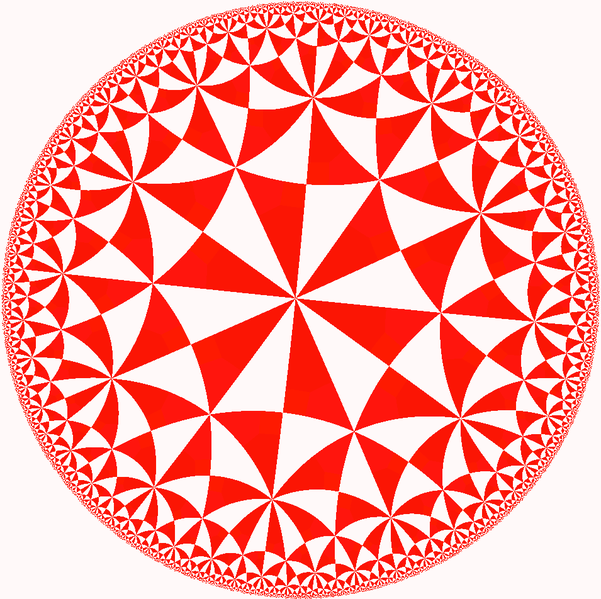
\includegraphics[width=\textwidth]{hyperbolic_domains}
            \caption{\textit{Afbeelding uit Coxeter's paper.}}
			\label{fig:hyperbolic-domains}
        \end{subfigure}%
       	~ 
        \begin{subfigure}{0.6\textwidth}
			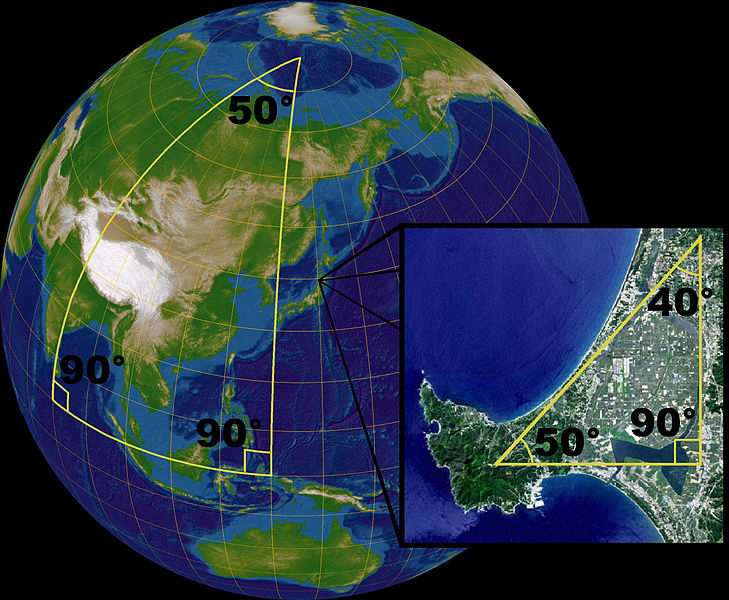
\includegraphics[width=\textwidth]{aarde}
            \caption{\textit{De aarde is een hyperbolische vlakte.}}
			\label{fig:aarde}
        \end{subfigure}%
        \caption{Hyperbolische vlaktes}
        \label{fig:structCompare}
\end{figure}

\end{document}
